%% -----------------------------------------------------------------
%% This file uses UTF-8 encoding
%%
%% For compilation use following command:
%% latexmk -pdf -pvc -bibtex --shell-escape thesis-manual
%% -----------------------------------------------------------------
\documentclass{kithesis}

% balicky
\usepackage[english,slovak]{babel}

% syntax higlighting and it's configuration
\usepackage{minted}  
\renewcommand\listoflistingscaption{Zoznam zdrojových kódov}
\renewcommand\listingscaption{Výpis}
\newminted{latex}{frame=lines,framerule=2pt}
\usemintedstyle{tango}

\usepackage{blindtext}  % lorem ipsum
\usepackage{nicefrac}  % pekne zlomky
\usepackage{rotating}  % umoznuje otacat obrazky spolu s popiskami
\usepackage{csquotes}

% premenne
\title{My master thesis \br with title over two lines}{Moja diplomová práca \br s názvom cez dva riadky}

\author{Janko Hraško}
\supervisor{Leslie Lamport} %veduciprace
\consultant{Donald E. Knuth} %konzultant
%\college{Žilinská univerzita}{Žilina} %univerzita
%\faculty{Fakulta elektrotechniky a informatiky} %fakulta
\department{Katedra počítačov a informatiky}{KPI} %katedra
%\thesis{Diplomová práca} %typprace
\submissiondate{13}{5}{2016}
%\fieldofstudy{9.2.1 Informatika}
%\studyprogramme{Informatika}
%\city{Košice} %mesto
\keywords{\LaTeX, programming, typesetting}{\LaTeX, programovanie, sadzba textu}
%\declaration{som nepodvadzal}

\abstract{%
    anglicky \LaTeX \blindtext
}{%
    slovensky \blindtext
}

\acknowledgment{Na tomto mieste by som rád poďakoval svojmu vedúcemu práce za jeho čas a odborné vedenie počas riešenia mojej záverečnej práce.

Rovnako by som sa rád poďakoval svojim rodičom a priateľom za ich podporu a povzbudzovanie počas celého môjho štúdia.
    
V neposlednom rade by som sa rád poďakoval pánom {\it Donaldovi E. Knuthovi} a {\it Leslie Lamportovi} za typografický systém \LaTeX, s ktorým som strávil množstvo nezabudnuteľných večerov.}

\addbibresource{thesis.bib}

% if you want to work only on selected chapters
%\includeonly{chapters/struktura} %,chapters/formatovanie}
%%%%%%%%%%%%%%%%%%%%%%%%%%%%%%%%%%%%%%%%%%%%%%%%%%%%%%%%%%%%%%%%%%%%%%%%%%%%%%%%
\begin{document}
%% Title page, abstract, declaration etc.:
\frontmatter{}

%% List of code listings
\listoflistings

% list of acronyms
\thispagestyle{empty}
% Acronyms
% ========
%
% An acronym is a word formed from the initial letters in a phrase. 
%
% Acronym Definition Exapmle:
% ---------------------------
% \newacronym{gcd}{GCD}{Greatest Common Divisor}
% \newacronym{dry}{DRY}{Don't Repeat Yourself}
%
% Usage:
% ------
% You can use these three options:
% 
% \acrlong{}  
%   Displays the phrase which the acronyms stands for. Put the label of the acronym inside the braces. In the example, \acrlong{gcd} prints Greatest Common Divisor. 
%
% \acrshort{} 
%   Prints the acronym whose label is passed as parameter. For instance, \acrshort{gcd} renders as GCD. 
%
% \acrfull{} 
%   Prints both, the acronym and its definition. In the example the output of \acrfull{dry} is Don't Repeat Yourself (DRY). 
% 
% For more information see:
% -------------------------
% * https://www.sharelatex.com/learn/Glossaries 
% * https://en.wikibooks.org/wiki/LaTeX/Glossary
%

\printglossary[type=\acronymtype,title={\acrlistname}]
\newpage

\pagenumbering{arabic}


%
\chapter{Inštalácia typografického systému\\ \LaTeX}
\label{ch:instalacia}

\section{Typografický systém \LaTeX}

Pre zvládnutie tohto jazyka neexistuje lepší spôsob, ako v ňom proste začať dokumenty rovno písať. Pre zvládnutie základov odporúčame použiť voľne dostupnú publikáciu \emph{The Not So Short Introduction to \LaTeX} \cite{lshort}, ktorú do slovenčiny preložili \emph{Ján Buša st.} a \emph{Ján Buša ml.} \cite{lshortsk}.

\section{Odporúčané balíčky}
\begin{itemize}
    \item \emph{minted}\footnote{\url{https://www.ctan.org/pkg/minted}} - zvýrazňovač zdrojového kódu (syntax highlighter) pre \LaTeX 
    \item \emph{europecv}\footnote{\url{https://www.ctan.org/pkg/europecv}} - šablóna pre písanie životopisov vo formáte EuroPass 
    \item \emph{PGF/TikZ}\footnote{\url{http://www.ctan.org/pkg/pgf}} - dvojica jazykov, pomocou ktorých je možné vytvárať vektorovú grafiku 
    \item \emph{rotating}\footnote{\url{https://www.ctan.org/pkg/rotating}} - umožňuje otáčať obrázky a tabuľky (spolu s ich popiskami)
\end{itemize}

\section{Inštalácia v OS Windows}

Ak pracujete v \emph{OS Windows}, stiahnite si distribúciu \LaTeX-u s názvom \emph{TeX Live} zo stránky \url{https://www.tug.org/texlive/}.

\section{Inštalácia v OS Linux}

Ak používate distribúciu \emph{Fedora 23}, pre používanie šablóny budete potrebovať nainštalovať nasledujúce balíčky:

\begin{minted}{bash}
$ sudo dnf install texlive-bibtopic texlive-cslatex \
                 texlive-collection-latex \
                 texlive-collection-fontsrecommended \
                 texlive-cite latexmk texlive-textcase \
                 texlive-engrec texlive-parskip \
                 texlive-minted \
                 texlive-europecv \
                 texlive-hyphen-english texlive-hyphen-slovak \
                 texlive-titlesec
\end{minted}


\section{Generovanie \LaTeX dokumentov}

Pre priame spúšťanie z príkazového riadku odporúčame použiť príkaz {\tt latexmk}, ktorý slúži na zostavenie  \LaTeX dokumentov. Príklad použitia je nasledovný:

\begin{minted}{bash}
$ latexmk -pdf -bibtex -shell-escape thesis
\end{minted}

Ak nechcete spúšťať tento príkaz zakaždým po vykonaní zmien v zdrojových súboroch, pridajte programu {\tt latexmk} prepínač {\tt -pvc}, ktorý zabezpečí ich sledovanie a znovuzostavenie výstupu automaticky:

\begin{minted}{bash}
$ latexmk -pdf -bibtex -shell-escape -pvc thesis
\end{minted}

Ak budete chcieť vyčistiť vygenerované výstupy, stačí nástroj {\tt latexmk} spustiť s prepínačom {\tt -c}:

\begin{minted}{bash}
$ latexmk -c thesis
\end{minted}

\chapter{Štruktúra záverečnej práce}
\label{ch:struktura}

Záverečná práca sa skladá z týchto častí:

\begin{enumerate}
    \item Predhovor
    \item Abstrakt
    \item Úvod práce
    \item Analytická časť práce
    \item Syntetická časť práce
    \item Vyhodnotenie
    \item Záver
	\item Prílohy
	\begin{itemize}
	    \item Životopis
	    \item Systémová príručka
	    \item Používateľská príručka
	\end{itemize}
\end{enumerate}

Záverečná práca musí obsahovať pôvodné myšlienky vytvorené autorom, nesmie byť len jednoduchým prerozprávaním známych faktov a postupov.

\section{Predhovor}

Predhovor v záverečnej práci nie je povinný. Ak je predhovor v práci uvedený, potom obsahuje dôvody pre
voľbu témy práce a pozadie realizácie práce.

\section{Abstrakt}

Abstrakt je stručný opis obsahu záverečnej práce. Z abstraktu musí byť čitateľovi zrejmé čo autor v práci
riešil (problém), ako to riešil (metódy), k čomu v práci dospel (výsledky) a aké sú prínosy jeho riešenia.

\section{Úvod práce}

Úvod práce stručne opisuje stanovený problém, kontext problému a motiváciu pre riešenie problému. Z úvodu by malo byť jasné, že stanovený problém doposiaľ nie je vyriešený a má zmysel ho riešiť. Súčasťou úvodu práce je formulácia úlohy (samostatná kapitola), v ktorej sú jasne stanovené ciele záverečnej práce na základe problému. V úvode neuvádzajte štruktúru práce, t.j. o čom je ktorá kapitola. Rozsah úvodu je minimálne 2 celé strany (vrátane formulácie úlohy). Jadro práce musí obsahovať analytickú, syntetickú a vyhodnocovaciu časť. Názvy jednotlivých kapitol a členenie jadra je ponechané na autora.
    
\section{Analytická časť práce}

Analytická časť záverečnej práce analyzuje existujúce podobné prístupy k riešeniu stanoveného problému. Autor práce musí uviesť v tejto časti existujúce prístupy a riešenia, pričom musí zaujať stanovisko k týmto prístupom a riešeniam a opísať ich výhody a nedostatky. Prevažne v tejto časti autor používa odkazy na použité zdroje. Autor v analýze nepreberá odseky z cudzích prác ale uvádza prevažne vlastné postoje podložené odkazmi na literatúru. Je odporúčané aby bola analýza podporená aj experimentmi ak to umožňuje téma práce (napr. vyskúšam softvér). Analytická časť tvorí zvyčajne \nicefrac{1}{4} jadra práce.

\section{Syntetická časť práce}

Syntetická časť opisuje metódy použité na syntézu riešenia a opisuje syntézu samotného riešenia (zvyčajne je to návrh/implementácia softvérového resp. hardvérového riešenia), pričom sa opiera o závery analytickej časti práce. Syntetická časť tvorí zvyčajne \nicefrac{1}{2} jadra práce.

\section{Vyhodnotenie}

Vyhodnocovacia časť je kľúčovou časťou záverečnej práce. Tato časť obsahuje vyhodnotenie navrhnutého (vytvoreného) riešenia. Uprednostňované je objektívne vyhodnotenie výsledkov práce, ktoré sa opiera o meranie a štatistické metódy, prípadne matematické dôkazy. V prípade nameraných hodnôt musí autor opísať metódu merania, priebeh merania, výsledky a interpretáciu výsledkov v kontexte riešeného problému a stanovených cieľov. Na základe vyhodnotenia riešenia autor opíše prínosy svojej práce. Vyhodnocovacia časť tvorí zvyčajne \nicefrac{1}{4} jadra práce.

\section{Záver}

Záver práce obsahuje zhrnutie výsledkov práce s jasným opisom prínosov a pôvodných (vlastných) výsledkov autora a vyhodnotenie splnenia stanovených cieľov. Je to stručné zhrnutie informácií uvedených v záverečnej práci. Záver by nemal obsahovať nové informácie. V závere by mal tiež autor poukázať na prípadné otvorené otázky, ktoré sú nad rámec rozsahu práce a mal by odporučiť ďalšie aktivity na pokračovanie pri riešení problému. Rozsah záveru je minimálne 1 celá strana.



% !TEX root = ../thesis-manual.tex

\chapter{Práca so šablónou}
\label{ch:sablona}

\section{Štruktúra projektu}

Projekt záverečnej práce má nasledovnú štruktúru:

\begin{verbatim}
.
|-- chapters
|   |-- analyza.tex
|   |-- bibliography.bib
|   |-- formulacia.tex
|   |-- motivacia.tex
|   |-- prilohaa.tex
|   |-- prilohy.tex
|   |-- synteza.tex
|   |-- vyhodnotenie.tex
|   `-- zaver.tex
|-- figures
|   `-- tugboat.png
|-- acronyms.tex
|-- kithesis.cls
`-- thesis.tex
\end{verbatim}

Význam jednotlivých súborov a priečinkov je nasledovný:

\begin{itemize}
    \item priečinok {\tt \bf{chapters/}} obsahuje {\tt .tex} súbory reprezentujúce samostatné kapitoly záverečnej práce. Ak niektorú z nich chcete do práce vložiť, môžete použiť príkaz \mint{latex}|\include{chapters/nazov.kapitoly}| V prípade, že chcete pracovať len na jednej alebo niektorých kapitolách a nechcete znovu generovať celú prácu, môžete využiť príkaz \mint{latex}|\includeonly{chapters/kapitola1,chapters/kapitola2}|
    \item priečinok {\tt \bf{figures/}} obsahuje zoznam obrázkov, ktoré boli v práci použité
    \item v súbore {\tt \bf{kithesis.cls}} sa nachádza samotná šablóna \emph{kpithesis}
    \item súbor {\tt \bf{chapters/bibliography.bib}} obsahuje zoznam literatúry vo formáte \emph{BibLaTeX}
    \item súbor {\tt \bf{acronyms.tex}} obsahuje zoznam skratiek, ktoré ste v práci použili
    \item súbor {\tt \bf{thesis.tex}} predstavuje hlavný súbor záverečnej práce
\end{itemize}


\section{Príkazy na nastavenie vlastností šablóny}

V šablóne je zadefinovaných niekoľko špeciálnych príkazov, pomocou ktorých je možné nastaviť vlastnosti výsledného dokumentu, ako napr. meno autora, názov univerzity, vlastné znenie poďakovania a pod. Niektoré príkazy majú dva povinné parametre, kde prvý nastavuje hodnotu príslušnej vlastnosti v anglickom jazyku a druhý nastavuje hodnotu príslušnej vlastnosti v slovenskom jazyku.

\subsection{Príkaz {\tt \textbackslash{}author}}

Pomocou tohto príkazu je možné nastaviť meno a priezvisko autora záverečnej práce. Jeho použitie je ilustrované v nasledovnom výpise kódu:

\begin{listing}[ht]
\begin{minted}[frame=lines]{latex}
\author{Juraj Matta}
\end{minted}
\caption{Nastavenie mena a priezviska autora záverečnej práce}
\end{listing}


\subsection{Príkaz {\tt \textbackslash{}title}}

Pomocou tohto príkazu je možné nastaviť názov záverečnej práce. 

Tento príkaz má dva parametre:
\begin{enumerate}
    \item názov práce v anglickom jazyku
    \item názov práce v slovenskom jazyku
\end{enumerate}

Jeho použitie je ilustrované v nasledovnom výpise kódu:

\begin{listing}[ht]
\begin{minted}[frame=lines]{latex}
\title{% english title
    Transportation of organic material over long distances
}{% slovak title
    Prenos organickej hmoty na veľké vzdialenosti
}
\end{minted}
\caption{Nastavenie názvu záverečnej práce}
\end{listing}

V prípade, že sa vám názov zalomí na titulnej strane nevhodne, môžete ho zalomiť sami pomocou pripraveného makra {\tt \textbackslash{}br} takto:

\begin{listing}[ht]
\begin{minted}[frame=lines]{latex}
\title{% english title
    Transportation of organic material\br{}over long distances
}{% slovak title
    Prenos organickej hmoty\br{}na veľké vzdialenosti
}
\end{minted}
\caption{Nastavenie názvu záverečnej práce cez dva riadky}
\end{listing}


\subsection{Príkaz {\tt \textbackslash{}college}}

Pomocou tohto príkazu je možné nastaviť názov univerzity, kde sa záverečná práca píše. Názov univerzity bude použitý na titulnej, ako aj na druhej strane záverečnej práce.

Tento príkaz má dva parametre:
\begin{enumerate}
    \item názov univerzity v anglickom jazyku
    \item názov univerzity v slovenskom jazyku
\end{enumerate}

Použitie tohto príkazu je ilustrované v nasledovnom výpise kódu:

\begin{listing}[ht]
\begin{minted}[frame=lines]{latex}
\college{% english title
    University of Žilina
}{% slovak title
    Žilinská univerzita
}
\end{minted}
\caption{Nastavenie názvu univerzity záverečnej práce}
\end{listing}

Tento príkaz je nepovinný. Ak ho v preambule práce nenastavíte, použije sa predvolená hodnota {\it Technická univerzita Košice} pre názov univerzity v slovenčine a {\it Technical university of Košice} pre názov univerzity v angličtine.


\subsection{Príkaz {\tt \textbackslash{}faculty}}

Tento príkaz slúži na nastavenie názvu fakulty, na ktorej záverečná práca vznikla. Názov sa následne použije na titulnej a druhej strane záverečnej práce.

Tento príkaz má dva parametre:
\begin{enumerate}
    \item názov fakulty v anglickom jazyku
    \item názov fakulty v slovenskom jazyku
\end{enumerate}

Použitie tohto príkazu je ilustrované v nasledovnom výpise kódu:

\begin{listing}[ht]
\begin{minted}[frame=lines]{latex}
\faculty{% english title
    Faculty of Metallurgy
}{% slovak title
    Hutnicka fakulta
}
\end{minted}
\caption{Nastavenie názvu fakulty záverečnej práce}
\end{listing}

Tento príkaz je nepovinný. Ak ho v preambule práce nenastavíte, použije sa predvolená hodnota {\it Fakulta elektrotechniky a informatiky} pre názov fakulty v slovenčine a {\it Faculty of Electrical Engineering and Informatics} pre názov fakulty v angličtine.


\subsection{Príkaz {\tt \textbackslash{}department}}

Pomocou tohto príkazu je možné nastaviť názov katedry, pod hlavičkou ktorej záverečná práca vznikla. Názov katedry sa zobrazí na titulnej, ako aj na druhej strane záverečnej práce.

Tento príkaz má dva parametre:
\begin{enumerate}
    \item názov katedry v anglickom jazyku
    \item názov katedry v slovenskom jazyku
\end{enumerate}

Použitie tohto príkazu je ilustrované v nasledovnom výpise kódu:

\begin{listing}[ht]
\begin{minted}[frame=lines]{latex}
\department{% english title
    Department of Cybernetics and Artificial Intelligence
}{% slovak title
    Katedra kybernetiky a umelej inteligencie
}
\end{minted}
\caption{Nastavenie názvu katedry}
\end{listing}

Tento príkaz je nepovinný. Ak ho v preambule práce nenastavíte, použije sa predvolená hodnota {\it Katedra počítačov a informatiky} pre názov katedry v slovenčine a {\it Department of Computers and Informatics} pre názov katedry v angličtine.


\subsection{Príkaz {\tt \textbackslash{}departmentacr}}

Pomocou tohto príkazu je možné nastaviť skratku katedry, resp. pracoviska, pod hlavičkou ktorého záverečná práca vznikla.

Tento príkaz má dva parametre:
\begin{enumerate}
    \item skratka katedry, resp. pracoviska v anglickom jazyku
    \item skratka katedry, resp. v slovenskom jazyku
\end{enumerate}

Použitie tohto príkazu je ilustrované v nasledovnom výpise kódu:

\begin{listing}[ht]
\begin{minted}[frame=lines]{latex}
\departmentacr{DCAI}{KKUI}
\end{minted}
\caption{Nastavenie skratky katedry}
\end{listing}

Tento príkaz je nepovinný. Ak ho v preambule práce nenastavíte, použije sa predvolená hodnota {\it KPI} pre skratku katedry resp. pracoviska v slovenčine a {\it DCI} pre skratku katedry resp. pracoviska v angličtine.

\subsection{Príkaz {\tt \textbackslash{}supervisor}}

Pomocou tohto príkazu je možné nastaviť meno a priezvisko vedúceho záverečnej práce. Jeho použitie je ilustrované v nasledovnom výpise kódu:

\begin{listing}[ht]
\begin{minted}[frame=lines]{latex}
\supervisor{Leslie Lamport}
\end{minted}
\caption{Nastavenie mena a priezviska vedúceho práce}
\end{listing}


\subsection{Príkaz {\tt \textbackslash{}consultant}}

Pomocou tohto príkazu je možné nastaviť meno a priezvisko konzultanta záverečnej práce. Jeho použitie je ilustrované v nasledovnom výpise kódu:

\begin{listing}[ht!]
\begin{minted}[frame=lines]{latex}
\consultant{Donald E. Knuth}
\end{minted}
\caption{Nastavenie mena a priezviska konzultanta práce}
\end{listing}


\subsection{Príkaz {\tt \textbackslash{}fieldofstudy}}

Pomocou tohto príkazu je možné nastaviť štúdijný odbor. Jeho použitie je ilustrované v nasledovnom výpise kódu:

\begin{listing}[ht!]
\begin{minted}[frame=lines]{latex}
\fieldofstudy{1.2.3 Programovanie}
\end{minted}
\caption{Príklad použitia príkazu {\tt \textbackslash{}fieldofstudy} pre nastavenie štúdijného oboru}
\end{listing}

Ak typ štúdijného oboru nenastavíte, použije sa predvolená hodnota {\it 9.2.1. Informatika}.


\subsection{Príkaz {\tt \textbackslash{}studyprogramme}}

Pomocou tohto príkazu je možné nastaviť štúdijný program. Jeho použitie je ilustrované v nasledovnom výpise kódu:

\begin{listing}[ht!]
\begin{minted}[frame=lines]{latex}
\studyprogramme{Programovanie}
\end{minted}
\caption{Príklad použitia príkazu {\tt \textbackslash{}studyprogramme} pre nastavenie štúdijného programu}
\end{listing}

Ak štúdijný program nenastavíte, použije sa predvolená hodnota {\it Informatika}.


\subsection{Príkaz {\tt \textbackslash{}thesis}}

Pomocou tohto príkazu je možné nastaviť typ záverečnej práce, ako napr. {\it Bakalárska práca} alebo {\it Dizertačná práca}. 

Tento príkaz má dva parametre:
\begin{enumerate}
    \item typ záverečnej práce v anglickom jazyku
    \item typ záverečnej práce v slovenskom jazyku
\end{enumerate}

Jeho použitie je ilustrované v nasledovnom výpise kódu:

\begin{listing}[ht!]
\begin{minted}[frame=lines]{latex}
\thesis{% english title
    Master thesis
}{% slovak title
    Diplomová práca
}
\end{minted}
\caption{Nastavenie typu záverečnej práce}
\end{listing}

Tento príkaz je nepovinný. Ak ho v preambule práce nenastavíte, použije sa predvolená hodnota {\it Bakalárska práca} pre slovenčinu a {\it Bachelor thesis} pre angličtinu.


\subsection{Príkaz {\tt \textbackslash{}declaration}}

Pomocou tohto príkazu je možné nastaviť text čestného vyhlásenia autora záverečnej práce. Príklad nastavenia vlastného textu čestného vyhlásenia je nasledovný:

\begin{listing}[ht!]
\begin{minted}[frame=lines]{latex}
\declaration{
    Cestne skautske, ze som celu pracu napisal sam.
}
\end{minted}
\caption{Nastavenie testu čestného vyhlásenia}
\end{listing}

Ak text čestného vyhlásenia nenastavíte, použije sa automaticky hodnota {\it Vyhlasujem, že som záverečnú prácu vypracoval(a) samostatne s~použitím uvedenej odbornej literatúry.}


\subsection{Príkaz {\tt \textbackslash{}submissiondate}}

Pomocou tohto príkazu je možné nastaviť dátum odovzdania práce. Tento príkaz má tri pozičné parametre:

\begin{enumerate}
    \item {\it deň}
    \item {\it mesiac}
    \item {\it rok}
\end{enumerate}

Príklad nastavenia dátumu odovzdania je nasledovný:

\mint{latex}|\submissiondate{24}{12}{2016}|


\subsection{Príkaz {\tt \textbackslash{}abstract}}

Pomocou tohto príkazu je možné napísať abstrakt záverečnej práce v slovenskom a anglickom jazyku. Príkaz má dva pozičné parametre:

\begin{enumerate}
    \item {\it znenie abstraktu v anglickom jazyku}
    \item {\it znenie abstraktu v slovenskom jazyku}
\end{enumerate}

Príklad použitia tohto príkazu ilustruje nasledovný výpis:

\begin{listing}[ht!]
\begin{minted}[frame=lines]{latex}
\abstract{% english abstract
    This bachelor thesis is dedicated to the design and implementa-
    tion of teleportation system, which can be used to travel over
    huge distances in real-time. System was tested and later 
    installed at \emph{U.S.S. Enterprise}, where it is successfully
    used till today.
}{% slovak abstract
    Tato bakalarska praca sa venuje navrhu a implementacii telepor-
    tovacieho systemu, vdaka ktoremu je mozne prekonavat obrovske 
    vzdialenosti v realnom case. System bol otestovany a neskor na-
    sadeny na \emph{U.S.S. Enterprise}, kde sa s uspechom pouziva 
    dodnes.
}
\end{minted}
\caption{Zadanie abstraktu záverečnej práce}
\end{listing}


\subsection{Príkaz {\tt \textbackslash{}keywords}}

Pomocou tohto príkazu je možné zadať kľúčové slová charakterizujúce záverečnú prácu v slovenskom a anglickom jazyku. Príkaz má dva pozičné parametre:

\begin{enumerate}
    \item {\it kľúčové slová v anglickom jazyku}
    \item {\it kľúčové slová v slovenskom jazyku}
\end{enumerate}

Príklad použitia tohto príkazu ilustruje nasledovný výpis:

\begin{listing}[ht!]
\begin{minted}[frame=lines]{latex}
\keywords{% english keywords
    traveling, real-time, teleportation
}{% slovak keywords
    cestovanie, realny cas, teleportacia
}
\end{minted}
\caption{Zadanie kľúčových slov záverečnej práce}
\end{listing}


\subsection{Príkaz {\tt \textbackslash{}acknowledgment}}

Pomocou tohto príkazu je možné napísať vlastné poďakovanie do práce. Príklad použitia tohto príkazu ilustruje nasledovný výpis:

\begin{listing}[ht!]
\begin{minted}[frame=lines]{latex}
\acknowledgment{%
    Rad by som podakoval kapitanovi Kirkovi za moznost experimental-
    neho overenia vysledkov mojej prace na jeho lodi. Za rapidne 
    zredukovanie jeho posadky vdaka experimentom sa mu ospravedlnu-
    jem.
}
\end{minted}
\caption{Napísanie vlastného poďakovania do práce}
\end{listing}



%%%%%%%%%%%%%%%%%%%%%%%%%%%%%%%%%%%%%%%%%%%%%%%%%%%%%%%%%%%%%%%%%%%%%%%%%%%%%%%%
\section{Príkazy na vygenerovanie špeciálnych strán}

Šablóna obsahuje niekoľko príkazov, pomocou ktorých je možné vygenerovať niekoľko špeciálnych strán na základe hodnôt premenných nastavených pomocou príkazov uvedených v predchádzajúcej podkapitole. Pomocou týchto príkazov je možné vygenerovať napr. titulnú stranu záverečnej práce alebo špeciálne strany, na ktorých sa zobrazí text poďakovania alebo čestného vyhlásenia.

\subsection{Príkaz {\tt \textbackslash{}frontpage}}

Pomocou tohto príkazu dôjde k vygenerovaniu obálky záverečnej práce. Obsah stránky bude zložený z:

\begin{itemize}
    \item názvu univerzity,
    \item názvu fakulty,
    \item názvu záverečnej práce,
    \item typu záverečnej práce,
    \item roku publikovania, a
    \item mena a priezviska autora záverečnej práce.
\end{itemize}


\subsection{Príkaz {\tt \textbackslash{}titlepage}}

Tento príkaz vygeneruje titulnú stránku záverečnej práce. Obsah stránky bude zložený z:

\begin{itemize}
    \item názvu a mesta univerzity,
    \item názvu fakulty,
    \item názvu záverečnej práce,
    \item typu záverečnej práce,
    \item roku publikovania,
    \item mena a priezviska autora záverečnej práce,
    \item štúdijného programu a štúdijného oboru,
    \item školiaceho pracoviska, a
    \item mien vedúceho a konzultanta práce.
\end{itemize}


\subsection{Príkaz {\tt \textbackslash{}abstractpage}}

Tento príkaz vygeneruje stránku s abstraktom v slovenskom a anglickom jazyku. Súčasťou tejto stránky budú aj kľúčové slová v oboch jazykoch.


\subsection{Príkaz {\tt \textbackslash{}declarationpage}}

Tento príkaz vygeneruje stránku s čestným vyhlásením.


\subsection{Príkaz {\tt \textbackslash{}acknowledgmentpage}}

Tento príkaz vygeneruje stránku s poďakovaním.


\subsection{Príkaz {\tt \textbackslash{}frontmatter}}

Tento príkaz vo vašej práci vygeneruje naraz postupne tieto stránky:

\begin{enumerate}
    \item prednú stránku
    \item titulnú stránku
    \item stránku s abstraktom práce
    \item stránku s čestným vyhlásením
    \item stránku s poďakovaním
    \item obsah záverečnej práce
    \item zoznam obrázkov
    \item zoznam tabuliek
\end{enumerate}

Pokiaľ nepotrebujete vo svojej práci toto poradie nutne upraviť alebo zmeniť vzhľad týchto stránok, stačí, ak ako prvý príkaz vášho dokumentu bude práve príkaz \mint{latex}|\frontmatter|


\section{Príklad kostry záverečnej práce}

Pre začatie písania vašej záverečnej práce vám môže poslúžiť nasledovná kostra dokumentu. V tejto kostre sa nachádzajú len povinné parametre. Ak teda potrebujete nastaviť ďalšie vlastnosti vašej práce, môžete na to použiť niektorú z uvedených premenných.


\begin{listing}[ht!]
\begin{minted}[frame=lines]{latex}
\documentclass{kithesis}
\usepackage[slovak]{babel}

\title{Nazov prace}
\author{Juraj Hrdza}
\supervisor{Leslie Lamport}
\consultant{Donald E. Knuth}
\submissiondate{24}{12}{2016}

\abstract{%
    Znenie slovenskeho abstraktu prace.
}{%
    Thesis abstract in English.
}

\keywords{zoznam klucovych slov}{keywords in English}

\acknowledgment{Text vlastneho podakovania}

\addbibresource{thesis.bib}

\begin{document}
\frontmatter{}
\chapter*{Motivácia}
\addcontentsline{toc}{chapter}{Motivácia}

\Blindtext

\section{Anal\'yza}

Text záverečnej práce obsahuje kapitolu, v~rámci ktorej autor uvedie
analýzu riešených problémov. Táto kapitola môže byť v~prípade potreby
delená do viacerých podkapitol. Autor v~texte záverečnej práce môže
zvýrazniť kľúčové slová, pričom sa použije príslušný štýl pre kľúčové
slová -- napr. toto je kľúčové slovo. V~texte môžu byť použité obrázky
a~tabuľky podľa nasledujúcich príkladov:

\begin{figure}[!ht]
\centering \unitlength=1mm
\begin{picture}(30,30)(0,0)
\put(0,0){\line(1,0){30}}
\put(0,0){\line(0,1){30}}
\put(30,0){\line(0,1){30}}
\put(0,30){\line(1,0){30}}
\end{picture}
\caption{Toto je štvorec}\label{o:1}
\end{figure}


Obrázok by mal byť podľa možnosti centrovaný. Pri jeho opisovaní
v~texte treba použiť odkazy na obrázok v~tvare Obrázok~\ref{o:1}.

\tabcolsep=8pt
\begin{table}[!ht]\caption{Prehľad jednotiek}\label{t:1}
\smallskip
\centering
\begin{tabular}{|l|c|} \hline
Názov	& (Jednotka v~sústave SI) \\ \hline
Napätie & $\upmu$V \\ \hline
\end{tabular}
\end{table}
\nomenclature{$\upmu$}{mikro, $10^{-6}$}
\nomenclature{SI}{Syst\`eme International}
\nomenclature{V}{volt, základná jednotka napätia v sústave SI}

Tabuľka by mala byť podľa možnosti centrovaná. Pri jej opisovaní
v~texte treba použiť odkazy na tabuľku v~tvare: pozri
Tabuľku~\ref{t:1}. Na číslovanie obrázkov, resp. tabuliek treba použiť
triedenie. Za slovom {\it Obrázok} nasleduje ako prvé číslo kapitoly
alebo časti, v~ktorej sa obrázok nachádza, potom medzera, pomlčka,
medzera a~poradové číslo ilustrácie v~danej kapitole alebo časti.
Napr.:~Obrázok~\ref{o:1} (čiže: prvý obrázok v~druhej kapitole alebo
časti). V~prípade, ak tabuľka presahuje stranu, je možné použiť balík
\verb+longtable+.

Navrhujeme zaraďovať obrázky v~elektronickej podobe. Napríklad
Obrázok~\ref{o:2}, ktorý opisuje riešenie diferenciálnej rovnice
tlmených oscilácií
%% \def\ud{\mathrm{d}}
\begin{equation}\label{r:1}
\frac{\ud^2y}{\ud t^2}+\frac{\ud y}{\ud t}+y =0, \qquad y(0)=1, \quad
y\,'(0)=15,
\end{equation}
bol vytvorený v~MATLABe a~príkazom \texttt{print tlmosc.eps -f1
-deps2} bol uložený vo formáte Encapsulated Postscript. Na prípadné
použitie pdf\LaTeX{}u sa obrázok konvertuje do formátu PDF, napr.
pomocou programu \texttt{epstopdf}. Zvyčajne sa číslujú vzťahy, na
ktoré sa v~texte odvolávame. Napríklad: vzťahy (\ref{r:1}) definujú
Cauchyho začiatočnú úlohu.


\begin{figure}[ht!]
\centering
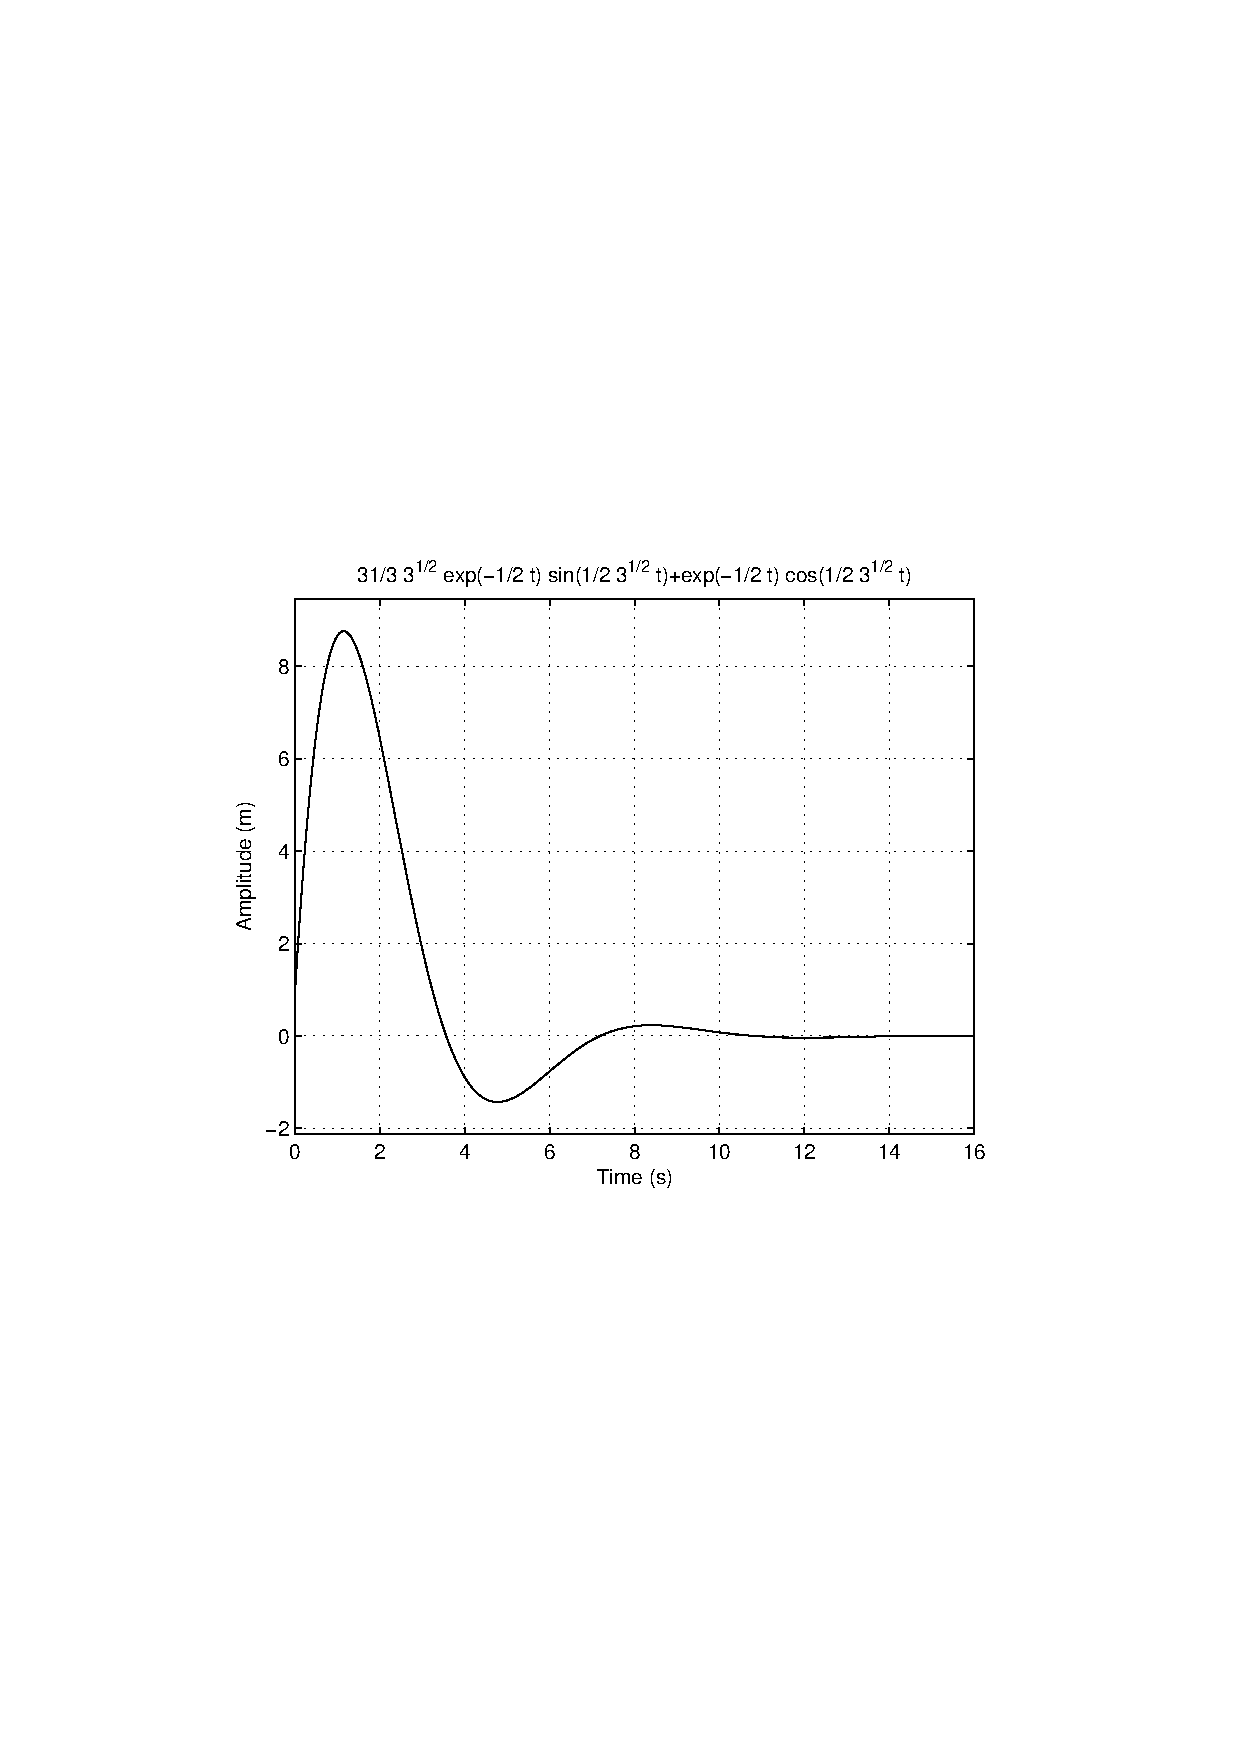
\includegraphics[width=0.7\textwidth]{tlmosc}
\caption{Grafické zobrazenie riešenia rovnice \ref{r:1}}\label{o:2}
\end{figure}



\subsection{Podkapitola}
Podkapitoly záverečnej práce majú za úlohu členenie textu záverečnej
práce s~cieľom, čo najväčšej prehľadnosti. Kapitol môže byť viacero
a~v~ich názvoch sa používa desatinné číslovanie.



\subsection{Vkladanie obrázkov}

Všetky obrázky, ktoré budete chcieť v dokumente použiť, ukladajte do priečinku {\tt figures/}. Následne obrázok vložte v prostredí \verb!figure! pomocou príkazu \verb!\includegraphics! bez uvedenia jeho prípony. Napríklad takto:

\begin{minted}{latex}
\begin{figure}[!ht]
	\centering
	
\includegraphics[width=\textwidth]{tugboat}
	\caption{\LaTeX{} priateľská zóna \label{o:latex\_friendly\_zone}}
\end{figure}

	\caption{Vloženie obrázku do textu dokumentu}
\end{minted}



\begin{figure}[!ht]
	\centering
	
\includegraphics[width=\textwidth]{tugboat}
	\caption{\LaTeX{} priateľská zóna \label{o:latex_friendly_zone}}
\end{figure}

\include{chapters/navrh}
\include{chapters/realizacia}
% !TEX root = ../thesis.tex

\chapter{Vyhodnotenie}

% lorem ipsum
\blindtext
\blinditemize
\Blindtext
\Blindtext

% !TEX root = ../thesis.tex

\chapter{Záver}

% lorem ipsum
\Blindtext


\printbibliography[title={Literatura}]
\end{document}

\end{minted}
\caption{Kostra dokumentu záverečnej práce}
\end{listing}

\chapter{Formátovanie dokumentu}

\section{Štruktúra projektu}

Projekt záverečnej práce má nasledovnú štruktúru:

\begin{verbatim}
.
|-- bibliography.bib
|-- CHANGELOG.md
|-- chapters
|   |-- formatovanie.tex
|   |-- instalacia.tex
|   `-- struktura.tex
|-- figures
|   |-- foto.png
|   `-- tugboat.png
|-- kpithesis.cls
`-- thesis.tex
\end{verbatim}

Význam jednotlivých súborov a priečinkov je nasledovný:

\begin{itemize}
    \item súbor {\tt \bf{bibliography.bib}} obsahuje zoznam literatúry vo formáte \emph{BibTeX}
    \item priečinok {\tt \bf{chapters/}} obsahuje {\tt .tex} súbory reprezentujúce samostatné kapitoly záverečnej práce
    \item priečinok {\tt \bf{figures/}} obsahuje zoznam obrázkov, ktoré boli v práci použité
    \item v súbore {\tt \bf{kpithesis.cls}} sa nachádza samotná šablóna \emph{kpithesis}
    \item súbor {\tt \bf{thesis.tex}} predstavuje hlavný súbor záverečnej práce
\end{itemize}


\section{Vkladanie obrázkov}

Všetky obrázky, ktoré budete chcieť v dokumente použiť, ukladajte do priečinku {\tt figures/}. Následne obrázok vložte do dokumentu pomocou prostredia \verb!figure! pomocou príkazu \verb!\includegraphics! bez uvedenia jeho prípony. Napríklad takto:

\begin{minted}{latex}
\begin{figure}[!ht]
    \centering
    
\includegraphics[width=\textwidth]{figures/tugboat}
    \caption{\LaTeX{} Friendly Zone \label{o:latex_friendly_zone}}
\end{figure}
\end{minted}

Výsledok tohto fragmentu kódu sa nachádza na obrázku \ref{o:latex_friendly_zone}.

\begin{figure}[!ht]
    \centering
    
\includegraphics[width=\textwidth]{figures/tugboat}
    \caption{\LaTeX{} Friendly Zone \label{o:latex_friendly_zone}}
\end{figure}

Ak chcete obrázok vložiť do dokumentu otočený o $90$, môžete použiť voľbu {\tt angle=90}, ktorú poskytuje balík {\tt graphicx}:

\begin{minted}{latex}
\begin{figure}[!ht]
    \centering
    
\includegraphics[angle=90,width=\textwidth]{figures/tugboat}
    \caption{\LaTeX{} Friendly Zone \label{o:latex_friendly_zone_90}}
\end{figure}
\end{minted}

Výsledkom tejto úpravy je obrázok \ref{o:latex_friendly_zone_90}.

\begin{figure}[!ht]
    \centering
    
\includegraphics[angle=90,width=\textwidth]{figures/tugboat}
    \caption{\LaTeX{} Friendly Zone \label{o:latex_friendly_zone_90}}
\end{figure}

V prípade, ak chcete otočiť obrázok spolu s popiskom, použite balíček {\tt rotating}, ktorý poskytuje prostredie {\tt sidewaysfigure} nasledovným spôsobom:

\begin{minted}{latex}
\begin{sidewaysfigure}
    \centering
    
\includegraphics[width=.7\textheight]{figures/tugboat}
    \caption{\LaTeX{} Friendly Zone \label{o:latex_friendly_zone_rotating}}
\end{sidewaysfigure}
\end{minted}

Výsledok tohto fragmentu kódu sa nachádza na obrázku \ref{o:latex_friendly_zone_rotating}.

\begin{sidewaysfigure}
    \centering
    
\includegraphics[width=.7\textheight]{figures/tugboat}
    \caption{\LaTeX{} Friendly Zone \label{o:latex_friendly_zone_rotating}}
\end{sidewaysfigure}

\section{Vkladanie tabuliek}

%%
%% !TEX root = ../thesis.tex

\chapter{Formulácia úlohy}

Text záverečnej práce musí obsahovať\/ kapitolu s~formuláciou úlohy resp. úloh riešených v~rámci záverečnej práce. V~tejto časti autor rozvedie spôsob, akým budú riešené úlohy a~tézy formulované v~zadaní práce. Taktiež uvedie prehľad podmienok riešenia.

%%
%\section{Anal\'yza}

Text záverečnej práce obsahuje kapitolu, v~rámci ktorej autor uvedie
analýzu riešených problémov. Táto kapitola môže byť v~prípade potreby
delená do viacerých podkapitol. Autor v~texte záverečnej práce môže
zvýrazniť kľúčové slová, pričom sa použije príslušný štýl pre kľúčové
slová -- napr. toto je kľúčové slovo. V~texte môžu byť použité obrázky
a~tabuľky podľa nasledujúcich príkladov:

\begin{figure}[!ht]
\centering \unitlength=1mm
\begin{picture}(30,30)(0,0)
\put(0,0){\line(1,0){30}}
\put(0,0){\line(0,1){30}}
\put(30,0){\line(0,1){30}}
\put(0,30){\line(1,0){30}}
\end{picture}
\caption{Toto je štvorec}\label{o:1}
\end{figure}


Obrázok by mal byť podľa možnosti centrovaný. Pri jeho opisovaní
v~texte treba použiť odkazy na obrázok v~tvare Obrázok~\ref{o:1}.

\tabcolsep=8pt
\begin{table}[!ht]\caption{Prehľad jednotiek}\label{t:1}
\smallskip
\centering
\begin{tabular}{|l|c|} \hline
Názov	& (Jednotka v~sústave SI) \\ \hline
Napätie & $\upmu$V \\ \hline
\end{tabular}
\end{table}
\nomenclature{$\upmu$}{mikro, $10^{-6}$}
\nomenclature{SI}{Syst\`eme International}
\nomenclature{V}{volt, základná jednotka napätia v sústave SI}

Tabuľka by mala byť podľa možnosti centrovaná. Pri jej opisovaní
v~texte treba použiť odkazy na tabuľku v~tvare: pozri
Tabuľku~\ref{t:1}. Na číslovanie obrázkov, resp. tabuliek treba použiť
triedenie. Za slovom {\it Obrázok} nasleduje ako prvé číslo kapitoly
alebo časti, v~ktorej sa obrázok nachádza, potom medzera, pomlčka,
medzera a~poradové číslo ilustrácie v~danej kapitole alebo časti.
Napr.:~Obrázok~\ref{o:1} (čiže: prvý obrázok v~druhej kapitole alebo
časti). V~prípade, ak tabuľka presahuje stranu, je možné použiť balík
\verb+longtable+.

Navrhujeme zaraďovať obrázky v~elektronickej podobe. Napríklad
Obrázok~\ref{o:2}, ktorý opisuje riešenie diferenciálnej rovnice
tlmených oscilácií
%% \def\ud{\mathrm{d}}
\begin{equation}\label{r:1}
\frac{\ud^2y}{\ud t^2}+\frac{\ud y}{\ud t}+y =0, \qquad y(0)=1, \quad
y\,'(0)=15,
\end{equation}
bol vytvorený v~MATLABe a~príkazom \texttt{print tlmosc.eps -f1
-deps2} bol uložený vo formáte Encapsulated Postscript. Na prípadné
použitie pdf\LaTeX{}u sa obrázok konvertuje do formátu PDF, napr.
pomocou programu \texttt{epstopdf}. Zvyčajne sa číslujú vzťahy, na
ktoré sa v~texte odvolávame. Napríklad: vzťahy (\ref{r:1}) definujú
Cauchyho začiatočnú úlohu.


\begin{figure}[ht!]
\centering
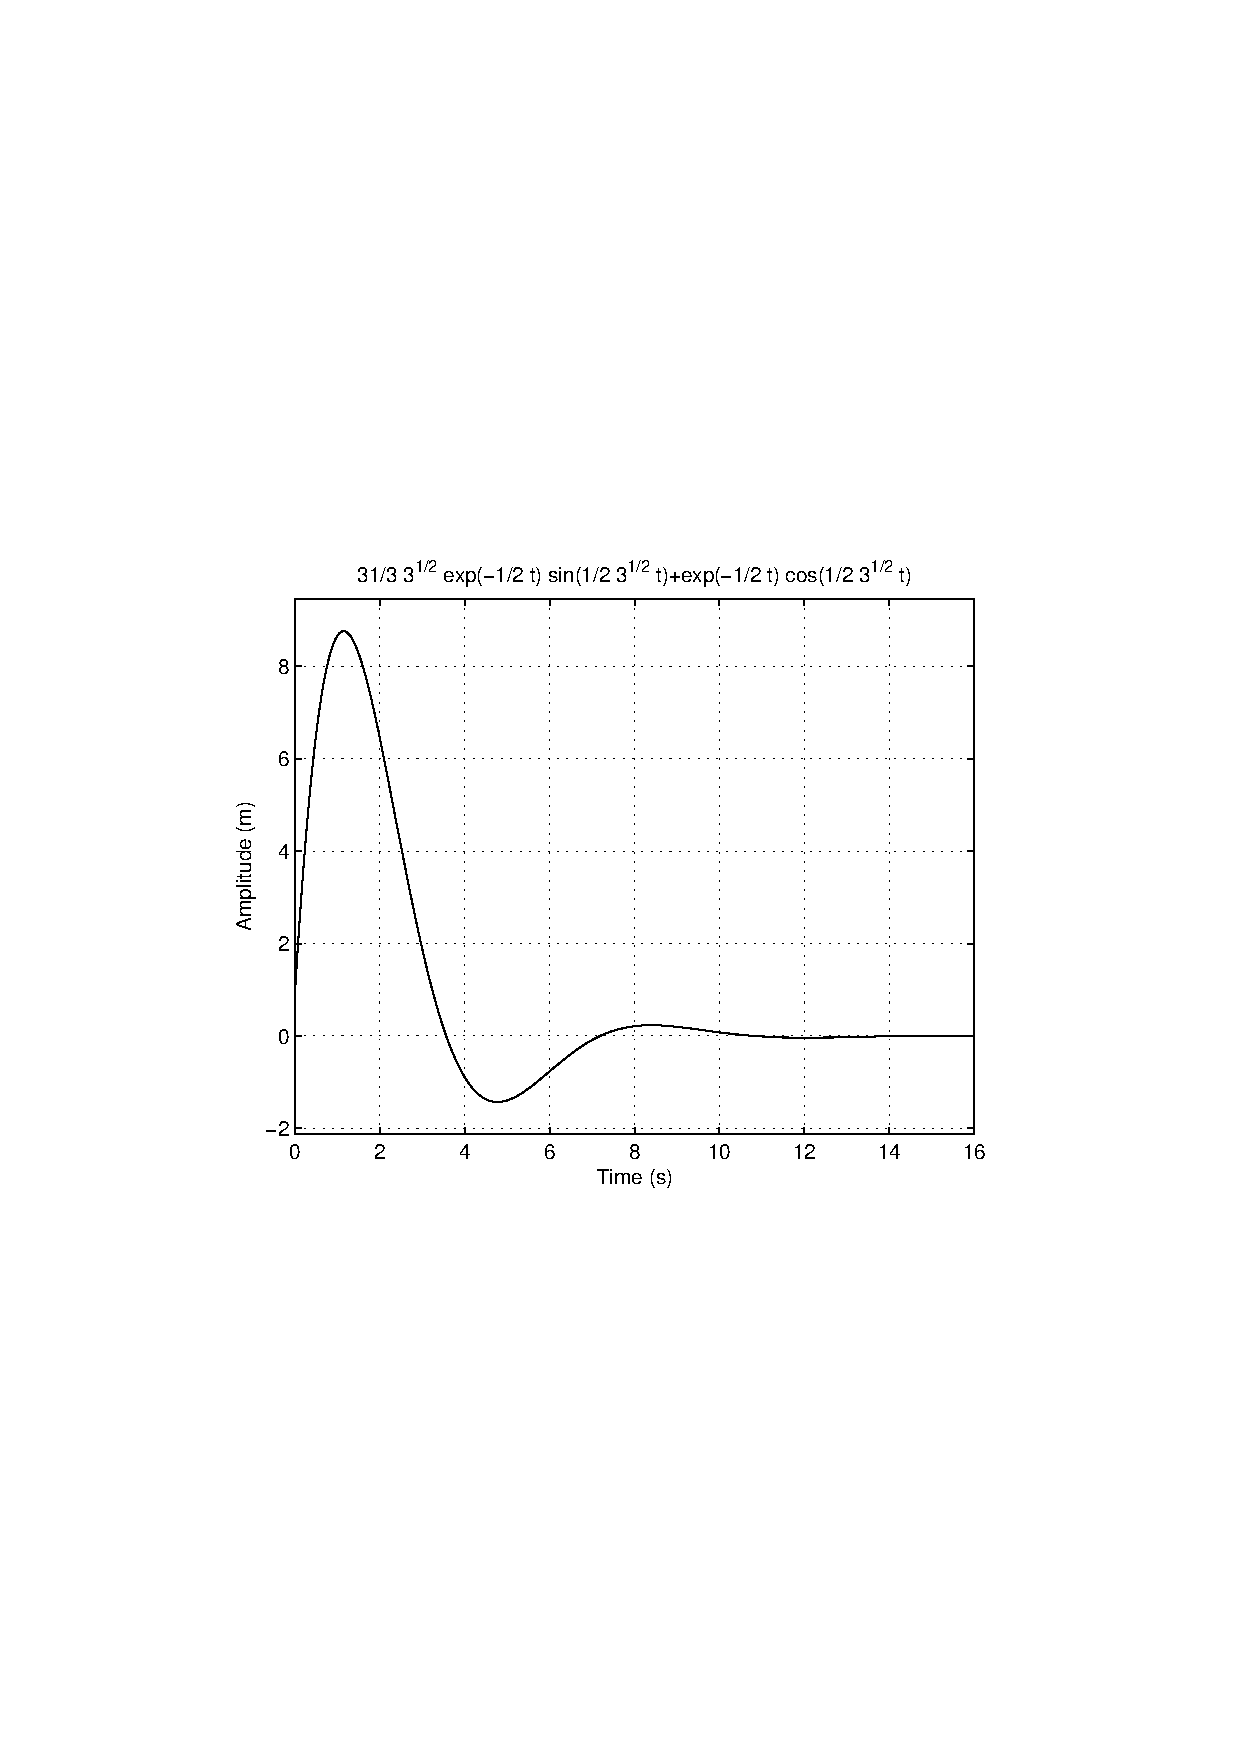
\includegraphics[width=0.7\textwidth]{tlmosc}
\caption{Grafické zobrazenie riešenia rovnice \ref{r:1}}\label{o:2}
\end{figure}



\subsection{Podkapitola}
Podkapitoly záverečnej práce majú za úlohu členenie textu záverečnej
práce s~cieľom, čo najväčšej prehľadnosti. Kapitol môže byť viacero
a~v~ich názvoch sa používa desatinné číslovanie.
%%
%\section{Jadro pr\'ace}

Začnime rovnicou

\begin{equation}\label{r:2}
\frac{\ud^2y}{\ud t^2}+\frac{\ud y}{\ud t}+y =0, \qquad y(0)=1, \quad
y\,'(0)=15.
\end{equation}

Grafický priebeh riešenia tejto rovnice vidíme na Obrázku \ref{o:2}.

\begin{figure}[ht!]
\centering
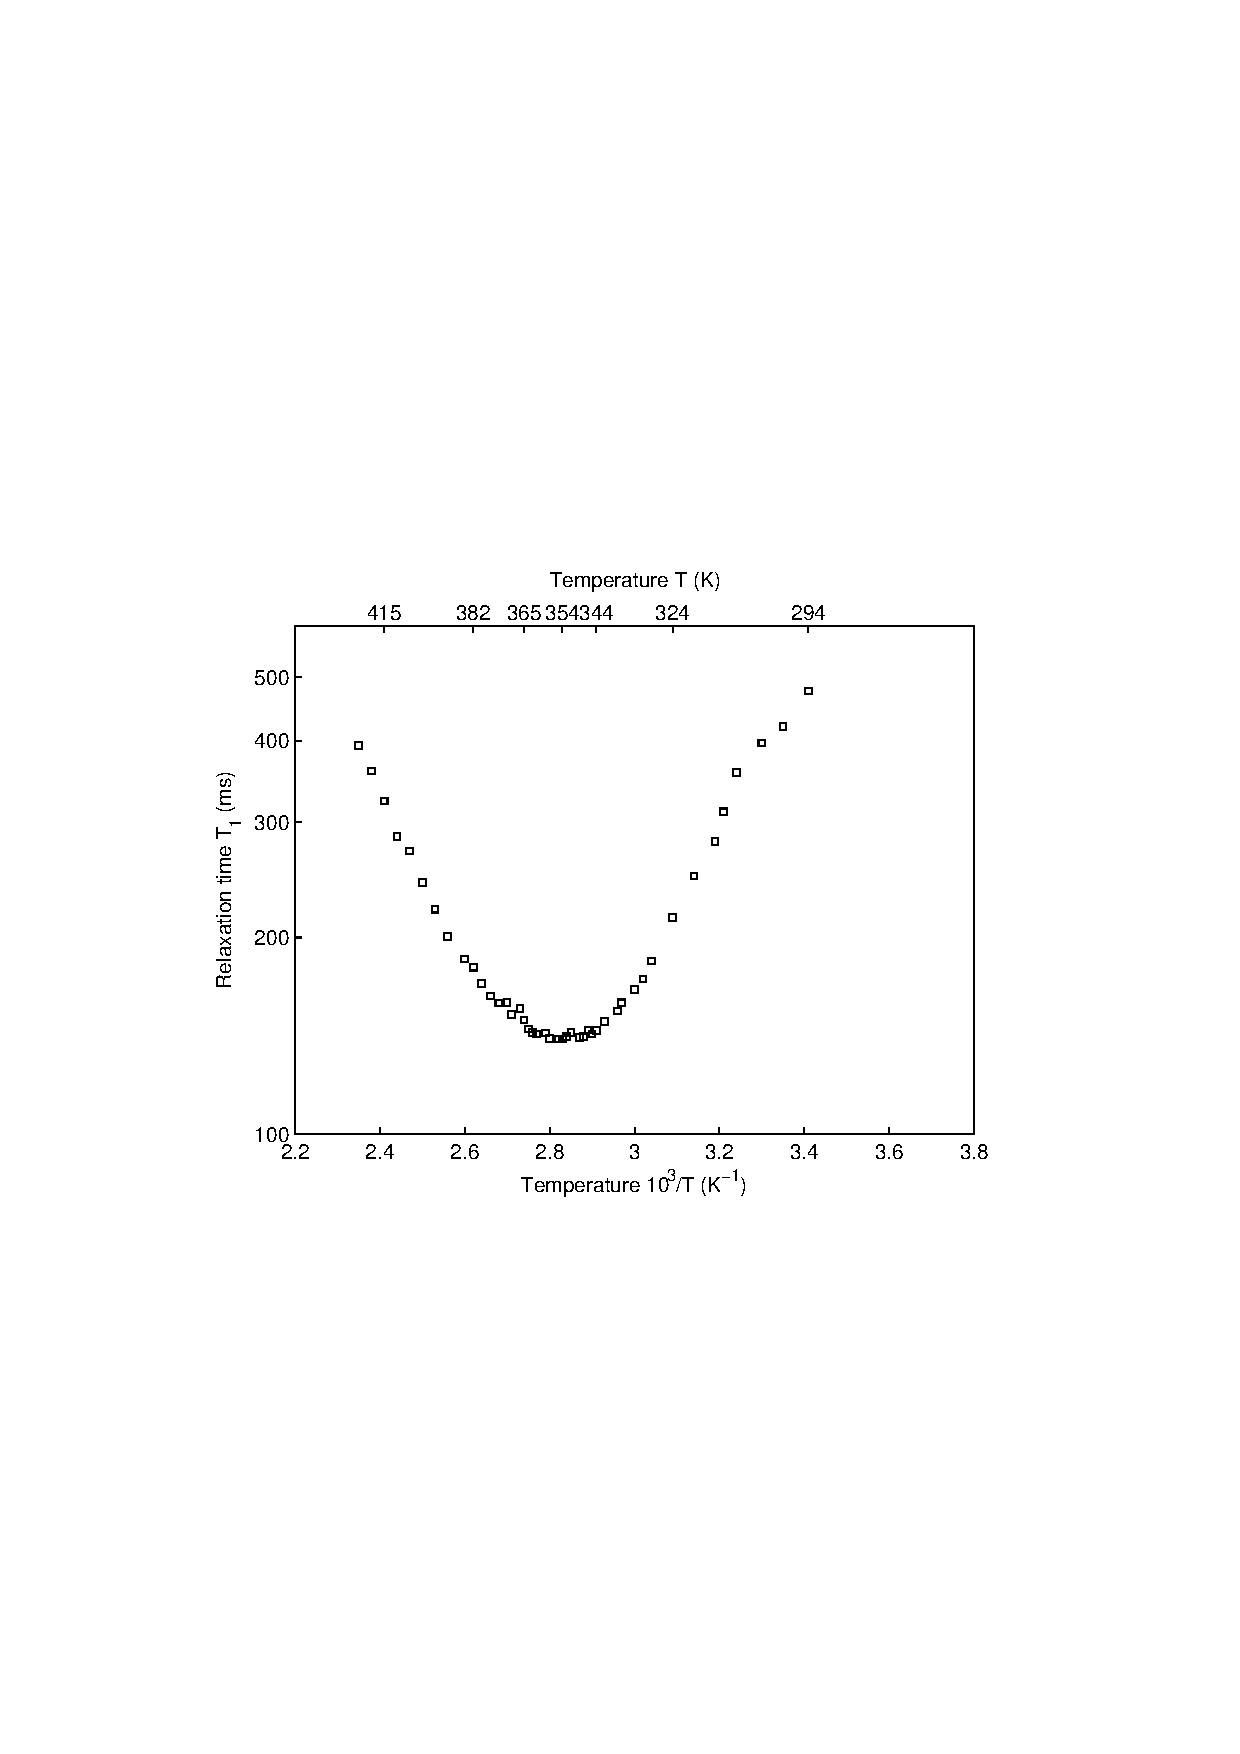
\includegraphics[width=.6\textwidth,angle=0]{relaxcas.pdf}
\caption{Teplotná závislosť\/ spinovo-mriežkového relaxačného
času}\label{o:3}
\end{figure}

%\tabcolsep=3pt % sirka stlpcov
%\renewcommand{\arraystretch}{1.2} % riadkovanie
\begin{table}[ht!]
\centering
\caption{Parametre získané z~meraní spinovo-mriežkových relaxačných
časov $T_1$}\label{t:2}
\medskip
\newcolumntype{d}{D{,}{,}{-1}}
\begin{tabular}{||c||d|d|d|d|d||}
\hhline{|t:==t:==:==:t|}
\multicolumn{1}{||c||}{}&\multicolumn{1}{c|}{PP --
01}&\multicolumn{1}{c|}{PP -- 05}&\multicolumn{1}{c|}{PP --
10}&\multicolumn{1}{c|}{PP -- 16}&\multicolumn{1}{c||}{PP -- 22} \\
\hhline{|:==:==:==:|}
C $\cdot 10^8$~(s$^{-2}$) & 10,1 & 10,0 & 11,0 & 9,2 & 8  \\
\hhline{||-|-|-|-|-|-||}
$\tau_0 \cdot 10^{-14}$~(s) & 2,63 & 1,44 & 0,95 & 2,21 & 10,83  \\
\hhline{||-|-|-|-|-|-||}
$E_{\text a}$~(kJ) & 34,26 & 8,33 & 39,76 & 37,31 & 31,86  \\
\hhline{||-|-|-|-|-|-||}
$T_{\min}$~(K) & 354 & 367 & 367 & 369 & 367  \\
\hhline{||-|-|-|-|-|-||}
$T_{1\min}$~(ms) & 141 & 160 & 157 & 175 & 181  \\
\hhline{||-|-|-|-|-|-||}
$\Delta M_2$~(Gs$^2$) & 5,49 & 5,66 & 5,16 & 5,09 & 5,02  \\
\hhline{|b:==b:==:==:b|}
\end{tabular}
\end{table}


%%
%% !TEX root = ../thesis.tex

\chapter{Záver}

% lorem ipsum
\Blindtext

%%
%%%
\begin{thebibliography}{999}
\addcontentsline{toc}{section}{\numberline{}Zoznam pou\v{z}itej
literat\'ury}

\harvarditem{Barančok et al.}{1995}{barancok}
BARANČOK, D. et al. 1995. \emph{The effect of semiconductor surface
treatment on LB film/Si interface.} In:~Physica Status Solidi (a), 
ISSN 0031-8965, 1995, vol. 108, no.~2, \mbox{pp. K~87--90}

\harvarditem{Benčo}{2001}{benco}
BENČO, J. 2001. \emph{Metodológia vedeckého výskumu.} Bratislava~:
IRIS, 2001, ISBN 80\discretionary{-}{-}{-}89018-27-0

\harvarditem{Gonda}{2001}{gonda}
GONDA, V. 2001. \emph{Ako napísať a~úspešne obhájiť diplomovú prácu.}
Bratislava~: Elita, 2001, 3. doplnené a~prepracované vydanie, 120~s.
ISBN 80-8044-075-1

\harvarditem{Jadr. fyz. a~tech.}{1985}{slovnik}
\emph{Jadrová fyzika a~technika: Terminologický výkladový slovník.}
2.~rev.~vyd. Bratislava~: ALFA, 1985. 235~s. ISBN 80-8256-030-5

\harvarditem{Katuščák}{1998}{kat}
KATUŠČÁK, D. 1998. \emph{Ako písať vysokoškolské a~kvalifikačné
práce.} Bratislava~: Stimul, 1998, 2.~doplnené vydanie. 121~s. ISBN
80-85697-82-3

\harvarditem{Lamoš a~Potocký}{1989}{lamos}
LAMOŠ, F. -- POTOCKÝ, R. 1989. \emph{Pravdepodobnosť a~matematická
štatistika.} 1.~vyd. Bratislava~: Alfa, 1989. 344~s. ISBN 80-8046-020-5

\harvarditem{Sýkora a~i.}{1980}{sykora}
SÝKORA, F. a~iní. 1980. \emph{Telesná výchova a~šport.} 1.vyd.
Bratislava~: SPN, 1980. 35~s. ISBN 80-8046-020-5

\harvarditem{Steinerová}{2000}{steinerova}
STEINEROVÁ, J. 2000. \emph{Základy filozofie človeka v~knižničnej
a~informačnej vede.} In:~Kimlička, Š., Knižničná a~informačná veda na
prahu informačnej spoločnosti. Bratislava~: Stimul, 2000. ISBN
80-2274-035-2, s. 327--334

\harvarditem{Šumichrast}{1995}{sumichrast}
ŠUMICHRAST, Ľ. 1995. \emph{On the performance of higher approximations
of radiation boundary conditions for the simulation of wave propagation
in structures of integrated optics.} In:~Photonics '95. Prague~: CTU,
1995, pp. 159--161
\end{thebibliography}
%\bibliographystyle{dcu}
%\bibliography{bibliography}{}
\printbibliography[title={Literatúra}]
%%
%\section*{Zoznam pr\'iloh}
\addcontentsline{toc}{section}{\numberline{}Zoznam pr\'iloh}
\thispagestyle{empty}

\begin{description}
	\item[Príloha A] Prílohy
	\item[Príloha B] Bibliografické odkazy
	\item[Príloha C] Vytvorenie zoznamu skratiek a symbolov
	\item[Príloha D] 
\end{description}
%%
%% !TEX root = ../thesis.tex

\chapter{Systémová príručka}
Táto časť slúži na opis priečinkov a rozdelenia kódu.
\section*{Rozdelenie kódu}
Funkčný kód je rozdelený na dve časti. Prvá časť sa venuje základnej úprave dát do čitateľnej formy, konkrétne vo funkcii main napísanej v kóde java. Druhá časť, ktorá klasifikuje všetky dáta, spracováva výsledky a vypočítava skóre, je napísaná v Pythone, konkrétne v main funkcii predict.py. 
\section*{Opis kódu}
Prvá časť v kóde main.java má dve funkcie. Je to funkcia GetCharFromString, ktorá vracia aktuálny charakter v stringu a funkcia main, v ktorej otvoríme ako BufferedReader textový súbor 'menochampiona'+1.txt a zároveň vytvoríme nový textový súbor 'menochampiona'+.txt. Následne prechádzame celý textový súbor a upravujeme ho do čitateľnej podoby.
\\ Druhá čast v kóde predict.py má dve hlavné priority. Prvá je zápis všetkých získaných textových súborov z programu javy do jedného dataframu a zároveň ich klasifikácia. A druhá pracuje s daným dataframom a počíta skóre.
\section*{Opis priečinkov}
V priečinku transformdata sa nachádza 332 súborov, z čoho je viac než 320 textových súborov s dátami o každom jednom šampiónovi. Zároveň je tam aj hlavná časť kódu a to súbor predict.py, ktorý má v sebe spracovanie a úpravu všetkých dát. Hlavný súbor s dátami sa volá winratedata.txt ktorý v sebe drží hodnoty všetkých klasifikovaných dát pre každého šampióna. Takisto v hlavnom priečinku môžete nájsť vysledky.xlsx, čo je excelovská tabuľka všetkých otestovaných zápasov. V priečinku src nájdeme kód main.java, pomocou ktorého sme dáta dostali do čitateľnej podoby pre náš python kód. 

\chapter{Používateľská príručka}
V tejto časti si ukážeme ako spustiť a obsluhovať aktuálny kód.

\section*{Potrebné súbory}
Na úspešné odskúšanie kódu na predikciu potrebujete mať textové súbory winratedata.txt, winlose.txt, teams.txt a zároveň samotný súbor s kódom predict.py, ktorý sa nachádza v hlavnom priečinku spolu s textovými súbormi.

\section*{Príprava prostredia a knižníc} 
Odporúčané prostredie je Spyder, ideálne verzia 5.0.5 a novšie. Prostredie Spyder je možné stiahnuť na ich domácej stránke zadarmo. Potrebná knižnica na stiahnutie je pandas, čo môžete vykonať príkazom - pip install pandas, napísaným v konzole.

\section*{Popis používania}
Kód predict.py je potrebné otvoriť v predpripravenom prostredí. Následne na vrchu kódu je 5 premenných top, jg, mid, bot a sup. Pri predikcii kompozície, ktorú chcete odskúšať do týchto premenných, vložte mená šampiónov bez medzier v ich mene s malými písmenami. Ak ste tak vykonali, spustite kód zelenou šípkou a v konzole by mali byť vypísané premenné totalgames, totalscore a známka, čo označuje aktuálnu kompozíciu, ktorú ste zapísali. 

%%
%\section*{Pr\'iloha B}
\addcontentsline{toc}{section}{\numberline{}Pr\'iloha B}
\subsection*{Bibliografick\'e odkazy}

Táto časť\/ záverečnej práce je povinná. V~zozname použitej literatúry
sa uvádzajú odkazy podľa normy STN~ISO~690--2 (01 0197) (Informácie
a~dokumentácia. Bibliografické citácie. Časť\/ 2: Elektronické
dokumenty alebo ich časti, dátum vydania 1.~12.~2001, ICS:~01.140.20).
Odkazy sa môžu týkať\/ knižných, časopiseckých a~iných zdrojov
informácií (zborníky z~konferencií, patentové dokumenty, normy,
odporúčania, kvalifikačné práce, osobná korešpondencia a~rukopisy,
odkazy cez sprostredkujúci zdroj, elektronické publikácie), ktoré boli
v~záverečnej práci použité.

Forma citácií sa zabezpečuje niektorou z~metód, opísaných v~norme
STN~ISO~690, 1998, s.~21. Podrobnejšie informácie nájdete na stránke
\texttt{http://www.tuke.sk/anta/} v~záložke {\small\sf Výsledky
práce/Prehľad normy pre publikovanie STN~ISO~690 a~STN~ISO~690-2}.

Existujú dva hlavné spôsoby citovania v~texte.

\begin{itemize}
\item Citovanie podľa mena a~dátumu.
\item Citovanie podľa odkazového čísla.
\end{itemize}

\emph{Preferovanou metódou citovania} v~texte vysokoškolskej
a~kvalifikačnej práce je podľa normy ISO~7144 citovanie podľa mena
a~dátumu \citep{kat,gonda}. V~tomto prípade sa zoznam použitej
literatúry upraví tak, že za meno sa pridá rok vydania. Na uľahčenie
vyhľadávania citácií sa zoznam vytvára v~abecednom poradí autorov.

\medskip

Príklad:
\dots podľa \citep{steinerova} je táto metóda dostatočne rozpracovaná
na to, aby mohla byť\/ všeobecne používaná v~\dots

\medskip

Druhý spôsob uvedenia odkazu na použitú literatúru je uvedenie len
čísla tohto zdroja v~hranatých zátvorkách bez mena autora (autorov)
najčastejšie na konci príslušnej vety alebo odstavca.

\medskip

Príklad:
\dots podľa [13] je táto metóda dostatočne rozpracovaná na to, aby
mohla byť\/ všeobecne používaná v~\dots ako je uvedené v~[14].

\medskip

Citácie sú spojené s~bibliografickým odkazom poradovým číslom v~tvare
indexu alebo čísla v~hranatých zátvorkách. Odkazy v~zozname na konci
práce budú usporiadané podľa týchto poradových čísel. Viacero citácií
toho istého diela bude mať\/ rovnaké číslo. Odporúča sa usporiadať\/
jednotlivé položky v~poradí citovania alebo podľa abecedy.

\medskip
\noindent
Rôzne spôsoby odkazov je možné dosiahnuť\/ zmenou voľby v~balíku
\verb+natbib+:

\noindent
\verb+% Citovanie podla mena autora a roku+\\
\verb+\usepackage[]{natbib}\citestyle{chicago}+\\
\verb+% Možnosť rôznych štýlov citácií. Príklady sú uvedené+\\
\verb+% v preambule súboru natbib.sty.+\\
\verb+% Napr. štýly chicago, egs, pass, anngeo, nlinproc produkujú+\\
\verb+% odkaz v tvare (Jones, 1961; Baker, 1952). V prípade, keď+\\
\verb+% neuvedieme štýl citácie (vynecháme \citestyle{}) v "options"+\\
\verb+% balíka natbib zapíšeme voľbu "colon".+

\medskip
\noindent
Keď zapneme voľbu \verb+numbers+, prepneme sa do režimu citovania
podľa odkazového čísla.

\noindent
\verb+% Metoda ciselnych citacii+\\
\verb+\usepackage[numbers]{natbib}+

\bigskip

Pri zápise odkazov sa používajú nasledujúce pravidlá:

V~odkaze na knižnú publikáciu (pozri príklad zoznamov na konci tejto
časti):
\begin{itemize}
\item Uvádzame jedno, dve alebo tri prvé mená oddelené pomlčkou,
ostatné vynecháme a~namiesto nich napíšeme skratku et al. alebo a~i.
\item Podnázov sa môže zapísať\/ vtedy, ak to uľahčí identifikáciu
dokumentu. Od názvu sa oddeľuje dvojbodkou a~medzerou.
\item Dlhý názov sa môže skrátiť\/ v~prípade, ak sa tým nestratí
podstatná informácia. Nikdy sa neskracuje začiatok názvu. Všetky
vynechávky treba označiť\/ znamienkami vypustenia  \uv{\dots}
\end{itemize}

Pri využívaní informácií z~elektronických dokumentov  treba
dodržiavať\/ tieto zásady:
\begin{itemize}
\item  uprednostňujeme autorizované súbory solídnych služieb
a~systémov,
\item zaznamenáme dostatok informácií o~súbore tak, aby ho bolo opäť\/
možné vyhľadať\/,
\item urobíme si kópiu použitého prameňa v~elektronickej alebo
papierovej forme,
\item za verifikovateľnosť\/ informácií zodpovedá autor, ktorý sa na
ne odvoláva.
\end{itemize}

Pre zápis elektronických dokumentov platia tie isté pravidlá, ako pre
zápis \uv{klasických}. Navyše treba uviesť\/ tieto údaje:
\begin{itemize}
\item  druh nosiča  [online], [CD-ROM], [disketa], [magnetická páska]
\item dátum citovania  (len pre online dokumenty)
\item dostupnosť\/  (len pre online dokumenty)
\end{itemize}

Poradie prvkov odkazu je nasledovné:
Autor. Názov. In Názov primárneho zdroja: Podnázov. [Druh  nosiča].
Editor. Vydanie alebo verzia. Miesto vydania : Vydavateľ, dátum
vydania. [Dátum citovania]. Poznámky.  Dostupnosť\/. ISBN alebo ISSN.
%%
%\section*{Pr\'iloha C}
\addcontentsline{toc}{section}{\numberline{}Pr\'iloha C}
\subsection*{Vytvorenie zoznamu skratiek a symbolov}

Ak sú v~práci skratky a symboly, vytvára sa \emph{Zoznam skratiek
a~symbolov} (a~ich dešifrovanie). V~prostredí \LaTeX{}u sa takýto
zoznam
ľahko vytvorí pomocou balíka \verb+nomencl+. Postup je nasledovný:
\begin{enumerate}
\item Do preambuly zapíšeme nasledujúce príkazy\\
\verb+\usepackage[slovak,noprefix]{nomencl}+\\ \verb+\makeglossary+
\item  V~mieste, kde má byť\/ vložený zoznam zapíšeme príkaz\\
\verb+\printglossary+
\item V miestach, kde sa vyskytujú skratky a symboly ich definíciu
zavedieme, napr. ako     	v~našom texte, príkazmi\\
\verb+\nomenclature{$\upmu$}{mikro, $10^{-6}$}+\\
\verb+\nomenclature{V}{volt, základná jednotka napätia v sústave SI}+\\
a dokument \uv{pre\LaTeX{}ujeme}.
\item Z~príkazového riadka spustíme program \verb+makeindex+
s~prepínačmi podľa použitého operačného systému, napr.~v~OS~GNU/Linux
s~distribúciou Ubuntu~$10.04$ a~verziou \verb+texlive 2009-7+
napíšeme:\\
\verb*+makeindex tukedip.glo -s nomencl.ist -o tukedip.gls+\\
~v~OS~Win\,XP s~verziou \verb+TeXLive 2010+
napíšeme:\\
\verb*+makeindex -o tukedip.gls -s nomencl.ist tukedip.glo+

\item Po opätovnom \uv{pre\LaTeX{}ovaní} dokumentu sa na
požadované
miesto vloží \emph{Zoznam skratiek a symbolov}.
\end{enumerate}

%
% zivotopis autora
%\curriculumvitae\protect
%\label{page:posledna}
%Táto časť\/ je nepovinná. Autor tu môže uviesť\/ svoje biografické
%údaje, údaje o~záujmoch, účasti na~projektoch, účasti na~súťažiach,
%získané ocenenia, zahraničné pobyty na~praxi, domácu prax, publikácie
%a~pod.

\end{document}
